\documentclass[border=10pt]{standalone}
\usepackage{amsmath}
\usepackage{amssymb}
\usepackage{tikz}
\usetikzlibrary{arrows.meta,calc,decorations.pathreplacing,patterns,shapes.geometric,positioning,shadings,3d}

\begin{document}
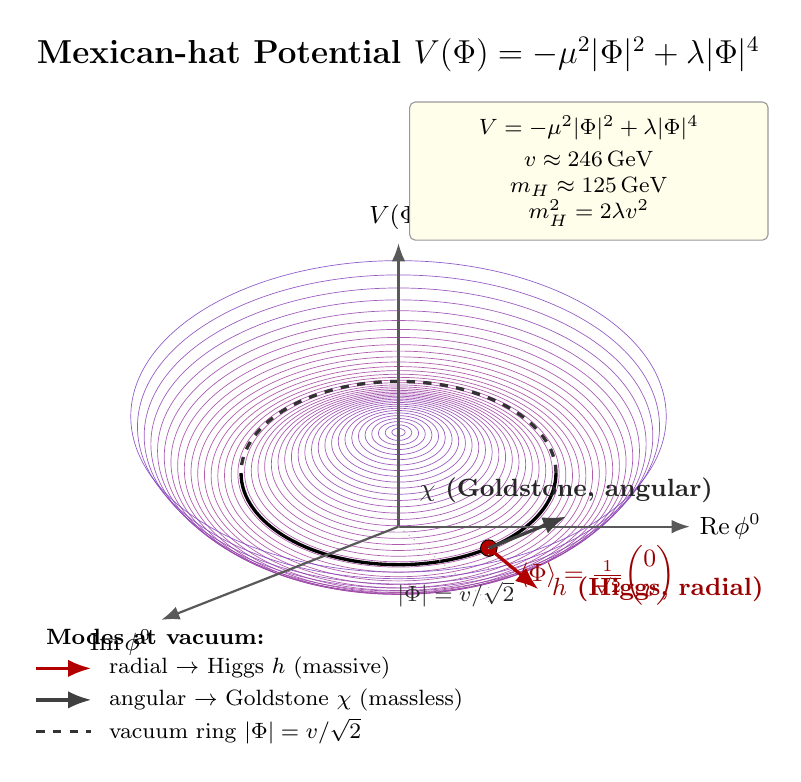
\begin{tikzpicture}[
  font=\small,
  >=Latex,
  scale=1.0,
  xax/.style={->, thick, gray!70!black},
  axislabel/.style={font=\small\itshape},
  vacring/.style={very thick, black!80, dashed},
  vacuum/.style={fill=red!70!black, draw=black, line width=0.3pt},
  higgsArrow/.style={->, very thick, red!70!black, line width=1.2pt},
  goldstoneArrow/.style={->, very thick, gray!50!black, line width=1.2pt}
]

% ----- Title -----
\node[font=\large\bfseries] at (0, 6.0) {Mexican-hat Potential $V(\Phi) = -\mu^2|\Phi|^2 + \lambda|\Phi|^4$};

% ============================================================
% Parameters
% ============================================================
% v/sqrt(2) chosen as ring radius (visual units = 2.0)
\def\Rv{2.0}              % vacuum radius
\def\Rmax{3.4}            % outer radius for surface
\def\hcenter{1.2}         % central hill height
\def\hbrim{2.6}           % outer brim height

% Depth/projection (3D into 2D)
\pgfmathsetmacro{\dx}{0.55}    % x-projection foreshortening
\pgfmathsetmacro{\dy}{0.32}    % y-projection foreshortening (depth into page)

% Helper: V(r) profile in plot coordinates (y is up).
% V_normalized(r) = a*r^4 - b*r^2 + c, with minimum at r=Rv, height = -a*Rv^4 ... we craft directly.

% ============================================================
% Draw the surface as stacked rings (back-to-front)
% Each ring at radius r is an ellipse at vertical position V(r)
% V(r) shape: small bump at center, valley at r=Rv, rising at r>Rv
% Use: V(r) = hbrim * ((r/Rmax)^4) - 2*hcenter*((r/Rmax)^2) + hcenter ... tuned manually
% ============================================================

% Draw filled "back-half" ellipses to create the surface look
% We'll layer many translucent rings.

\begin{scope}
  % Background sky
  % (none)

  % We draw filled ellipses at decreasing r (outermost first), to build the bowl from outside in.
  % Actually for proper 3D look (looking from above-front), we draw from BACK to FRONT,
  % which means draw smaller-r ellipses first if center is highest? No: we draw the OUTER rim first
  % (which is high), then inner valley, then center hill. Painter's algorithm: draw from back to front
  % in y. Since we project into xy-plane with y_screen = V(r) - dy*y_world, and the "back" of an ellipse
  % is its top edge in screen coords. To keep it simple and visually convincing, we'll shade by stacking
  % many thin ellipse outlines on top of each other.

  % Draw many circular contour lines, with their height giving V.
  \foreach \rstep in {0,1,...,40}{%
    \pgfmathsetmacro{\r}{\Rmax * \rstep / 40}
    % V profile
    \pgfmathsetmacro{\Vr}{\hbrim * pow(\r/\Rmax, 4) - 2*\hcenter*pow(\r/\Rmax, 2) + \hcenter}
    % color: blue at low V (valley), red at high V (rim/center hill)
    \pgfmathsetmacro{\cnorm}{(\Vr + \hcenter)/(\hbrim + \hcenter) * 100}
    % Determine color blend
    \pgfmathtruncatemacro{\cint}{\cnorm}
    %
    \pgfmathsetmacro{\elx}{\r}
    \pgfmathsetmacro{\ely}{\r * \dy / \dx}
    %
    % Draw circle at height \Vr using ellipse projection: center (0, \Vr), x-rad = r, y-rad = r*dy/dx
    \draw[draw=blue!\cint!red!75, line width=0.25pt, opacity=0.85]
      (0, \Vr) ellipse ({\elx} and {\ely});
  }
\end{scope}

% ============================================================
% Highlight the vacuum ring at r = Rv
% ============================================================
\pgfmathsetmacro{\Vmin}{\hbrim * pow(\Rv/\Rmax, 4) - 2*\hcenter*pow(\Rv/\Rmax, 2) + \hcenter}
\pgfmathsetmacro{\Rvy}{\Rv * \dy / \dx}

% Back half of the ring (dashed, behind)
\draw[vacring]
  (0, \Vmin) ++(\Rv, 0) arc[start angle=0, end angle=180, x radius=\Rv, y radius=\Rvy];
% Front half of the ring (solid, in front)
\draw[very thick, black]
  (0, \Vmin) ++(\Rv, 0) arc[start angle=0, end angle=-180, x radius=\Rv, y radius=\Rvy];

% ============================================================
% Axes (drawn at base of plot, y=0)
% ============================================================
% Origin at (0,0) base
\coordinate (O) at (0,0);
% Re axis (to the right, slightly down for 3D)
\coordinate (ReEnd) at ($(O)+({1.3*\Rmax}, {-0.05*\Rmax})$);
% Im axis (into page = up-left)
\coordinate (ImEnd) at ($(O)+({-1.0*\Rmax*\dy/\dx*1.3}, {-1.0*\Rmax*0.65*\dy/\dx*1.3 + 0.5})$);
% V axis (up)
\coordinate (Vend) at (0, {\hbrim + 1.0});

\draw[xax] (O) -- ($(O)+(\Rmax+0.3, 0)$);
\node[axislabel, anchor=west] at ($(O)+(\Rmax+0.3, 0)$) {$\mathrm{Re}\,\phi^0$};

% Im axis -- a diagonal going back into the page
\draw[xax] (O) -- ($(O)+({-(\Rmax+0.3)*\dy/\dx*1.4}, {-(\Rmax+0.3)*\dy/\dx*0.55})$);
\node[axislabel, anchor=north east] at ($(O)+({-(\Rmax+0.3)*\dy/\dx*1.4}, {-(\Rmax+0.3)*\dy/\dx*0.55})$) {$\mathrm{Im}\,\phi^0$};

% V axis (going up)
\draw[xax] (O) -- (0, \hbrim+1.0);
\node[axislabel, anchor=south] at (0, \hbrim+1.05) {$V(\Phi)$};

% ============================================================
% Vacuum point (red) on the front of the ring
% Place at angle theta = -50 deg around z (front-right)
% In our projection, point at angle theta on ring radius Rv at height Vmin:
%   x_screen = Rv*cos(theta)
%   y_screen = Vmin + Rv*sin(theta)*dy/dx    (sin>0 = back, sin<0 = front)
% Place at theta = -55 deg (front-right, visible)
% ============================================================
\pgfmathsetmacro{\thv}{-55}
\pgfmathsetmacro{\xV}{\Rv*cos(\thv)}
\pgfmathsetmacro{\yV}{\Vmin + \Rv*sin(\thv)*\dy/\dx}
\coordinate (VAC) at (\xV, \yV);

% Marker
\draw[vacuum] (VAC) circle (3pt);

% Label for VEV
\node[anchor=west, red!60!black, font=\small] at ($(VAC)+(0.25,-0.35)$)
  {$\langle\Phi\rangle = \frac{1}{\sqrt 2}\!\begin{pmatrix}0\\v\end{pmatrix}$};

% ============================================================
% Higgs (radial) and Goldstone (angular) arrows from VAC
% Radial direction in world: from origin outward in plane => screen (cos thv, sin thv*dy/dx)
% Angular (tangent) direction: perpendicular in plane => (-sin thv, cos thv*dy/dx)
% ============================================================
% Radial arrow length (along plane)
\pgfmathsetmacro{\Lrad}{1.1}
\pgfmathsetmacro{\xRad}{\Lrad*cos(\thv)}
\pgfmathsetmacro{\yRad}{\Lrad*sin(\thv)*\dy/\dx}
% Endpoint of radial arrow:
\coordinate (HRAD) at ($(VAC)+(\xRad, \yRad)$);

% Tangent arrow length
\pgfmathsetmacro{\Ltan}{1.2}
\pgfmathsetmacro{\xTan}{-\Ltan*sin(\thv)}
\pgfmathsetmacro{\yTan}{\Ltan*cos(\thv)*\dy/\dx}
\coordinate (GTAN) at ($(VAC)+(\xTan, \yTan)$);

\draw[higgsArrow] (VAC) -- (HRAD);
\draw[goldstoneArrow] (VAC) -- (GTAN);

% Labels for the modes
\node[red!60!black, anchor=west, font=\small\bfseries] at ($(HRAD)+(0.05,0.0)$) {$h$ (Higgs, radial)};
\node[gray!30!black, anchor=south, font=\small\bfseries] at ($(GTAN)+(0.0, 0.05)$) {$\chi$ (Goldstone, angular)};

% ============================================================
% Vacuum radius annotation
% Draw a small radial line from origin to VAC (projected onto base plane only)
% Place "|Phi|=v/sqrt(2)" label
% ============================================================
% Project VAC onto base plane (z=0) at (xV, sin(thv)*Rv*dy/dx)
\pgfmathsetmacro{\xVbase}{\Rv*cos(\thv)}
\pgfmathsetmacro{\yVbase}{\Rv*sin(\thv)*\dy/\dx}
\coordinate (VACbase) at (\xVbase, \yVbase);

% Small dotted line from origin in base plane to VACbase
\draw[dotted, gray!60] (O) -- (VACbase);
% Vertical dotted from VACbase up to VAC
\draw[dotted, gray!60] (VACbase) -- (VAC);

% Label for radius
\node[gray!30!black, font=\footnotesize, anchor=north] at ($(O)!0.55!(VACbase)+(0.1, -0.05)$)
  {$|\Phi|=v/\sqrt 2$};

% ============================================================
% Numbers / formula box (top right)
% ============================================================
\node[draw=black!40, fill=yellow!8, rounded corners=2pt, inner sep=5pt, anchor=north east, font=\footnotesize]
  at (4.7, 5.4)
{%
  \begin{minipage}{4.2cm}
    \centering
    $V=-\mu^2|\Phi|^2+\lambda|\Phi|^4$\\[2pt]
    $v\approx 246\,\mathrm{GeV}$\\
    $m_H\approx 125\,\mathrm{GeV}$\\
    $m_H^2 = 2\lambda v^2$
  \end{minipage}
};

% ============================================================
% Legend (bottom-left)
% ============================================================
\begin{scope}[shift={(-4.6,-2.0)}]
  \node[anchor=west, font=\footnotesize] at (0, 0.6) {\textbf{Modes at vacuum:}};
  \draw[higgsArrow] (0, 0.2) -- (0.7, 0.2);
  \node[anchor=west, font=\footnotesize] at (0.8, 0.2) {radial $\to$ Higgs $h$ (massive)};
  \draw[goldstoneArrow] (0, -0.2) -- (0.7, -0.2);
  \node[anchor=west, font=\footnotesize] at (0.8, -0.2) {angular $\to$ Goldstone $\chi$ (massless)};
  \draw[vacring] (0, -0.6) -- (0.7, -0.6);
  \node[anchor=west, font=\footnotesize] at (0.8, -0.6) {vacuum ring $|\Phi|=v/\sqrt 2$};
\end{scope}

\end{tikzpicture}
\end{document}
